% This is samplepaper.tex, a sample chapter demonstrating the
% LLNCS macro package for Springer Computer Science proceedings;
% Version 2.20 of 2017/10/04
%
\documentclass[runningheads]{llncs}
%
\usepackage{helvet,times,courier}
\usepackage{graphicx}
\usepackage{changepage}
\usepackage{cite}
\usepackage{algorithm}
\usepackage{algpseudocode}
\usepackage{mathtools}
\usepackage{rotating}
\usepackage{caption}
\usepackage{todonotes}
\usepackage[inline]{enumitem}
\captionsetup[table]{skip=10pt}
\DeclarePairedDelimiter\ceil{\lceil}{\rceil}
% Used for displaying a sample figure. If possible, figure files should
% be included in EPS format.
%
% If you use the hyperref package, please uncomment the following line
% to display URLs in blue roman font according to Springer's eBook style:
% \renewcommand\UrlFont{\color{blue}\rmfamily}

\newcommand{\stest}{\textit{ST\_EST}}
\newcommand{\stmtwr}{\textit{ST\_MTWR}}
\newcommand{\stfifo}{\textit{ST\_FIFO}}

\newcommand{\wtest}{\textit{WT\_EST}}
\newcommand{\wtmtwr}{\textit{WT\_MTWR}}
\newcommand{\wtfifo}{\textit{WT\_FIFO}}

\begin{document}
%
\title{Decomposition-based Job-shop Scheduling with Constrained Clustering}%\thanks{Supported by organization x.}}
%
\titlerunning{Decomposition-based JSP with Constrained Clustering}
% If the paper title is too long for the running head, you can set
% an abbreviated paper title here
%
\author{Mohammed M. S. El-Kholany\inst{1}\orcidID{0000-0002-1088-2081} \and
Konstantin Schekotihin\inst{1}\orcidID{0000-0002-0286-0958} \and
Martin Gebser\inst{1,2}\orcidID{0000-0002-8010-4752}}
%
\authorrunning{M. El-Kholany et al.}
% First names are abbreviated in the running head.
% If there are more than two authors, 'et al.' is used.
%
\institute{Alpen-Adria-Universität Klagenfurt, % Klagenfurt, 
Austria\\% 
% \email{\{mohammed.el-kholany, konstantin.schekotihin and martin.gebser\}@aau.at}%\\
%\url{http://www.springer.com/gp/computer-science/lncs}
\and
Technische Universität Graz, % Graz, 
Austria\\%
% \email{mgebser@ist.tugraz.at}
\email{firstname.lastname@aau.at}}
%
\maketitle              % typeset the header of the contribution
%
\begin{abstract}
Scheduling is a crucial problem appearing in various domains, such as manufacturing, transportation, or healthcare, where % . In most problem definitions, 
the goal is to schedule % a given set of 
given operations on available resources such that the operations are completed as soon as possible. Unfortunately, most scheduling problems cannot be solved efficiently, % Therefore, the 
so that research on suitable approximation methods is of primary importance.
%
This work introduces a novel approximation approach based on problem decomposition with data mining methodologies. We propose a constrained clustering algorithm to group operations into clusters, corresponding to time windows in which the operations must be scheduled. 
The decomposition process consists of two main phases. 
First, features are extracted, either from the problem itself or from solutions obtained by heuristic methods, to predict the execution sequence of operations on each resource.
% The first phase is to extract features to predict the sequence of operations on each resource. These features are extracted either from the problem itself or from solutions obtained by other heuristics.
The second phase % is to develop
deploys our constrained clustering algorithm to assign each operation into a time window. We then schedule the operations by time windows using Answer Set Programming. Evaluation results show that our proposed approach outperforms other heuristic schedulers in most cases, where incorporating features like \textit{Remaining Processing Time}, \textit{Machine Load}, and \textit{Earliest Starting Time} significantly improves the solution quality.

\keywords{Job-shop Scheduling  Problem \and Constrained Clustering \and Time Windows \and Answer Set Programming}
\end{abstract}
%
%
%
\section{Introduction}
Scheduling is one of the most crucial problems in various industrial, transportation, or healthcare applications
%\todo{add 1-2 citations for each application}
 \cite{pezzella2008genetic,chaudhry2016research,nouiri2018effective,demirbilek2019dynamically,schoenfelder2020nurse,wang2019routing,janakbhai2021blockchain}. 
%
Such applications result in different scheduling problem definitions, with the Job-shop Scheduling Problem (JSP) \cite{taillard1993benchmarks} being one if not the most well-known variant.
In JSP, operations of given jobs must be scheduled on available machines in an optimal way wrt.\ some pre-defined criteria. The latter include, for instance, minimization of makespan, i.e., the latest completion time of any job, or tardiness, i.e., the sum of delays over all jobs completed after their deadlines. 

However, JSP is an NP-complete combinatorial optimization problem \cite{DBLP:journals/mor/GareyJS76,SOTSKOV1995237} for which no efficient algorithms are known. Therefore, searching for an optimal solution with state-of-the-art solvers for Answer Set Programming (ASP), Mixed Integer Programming, or Constraint Programming \cite{meng2020mixed,coltep19a,el2020job,al2017job}
%\todo{cite at least 1 paper solving JSP with these methods} 
often takes too much computation time, even for seemingly small instances. Practical applications instead necessitate solving JSP instances of large scale with thousands of operations~\cite{zhang2010hybrid}.
As a result, much research work focuses on % the development of 
efficient methods for finding high-quality approximations of optimal schedules, including dispatching rules and other heuristic approaches~\cite{blackstone1982state} as well as stochastic optimization techniques \cite{DBLP:journals/informs/VaessensAL96,DBLP:journals/jim/CalisB15}.  
The main issue of these approaches is that they require manual parametrization for a particular scheduling problem, which is tedious and error-prone. For instance, adapting heuristic methods might involve the development of new dispatching rules or specific combinations of existing ones. Similarly, merely utilizing default parameters for stochastic techniques might lead to mediocre schedules.    
In view of these challenges, recent research interest lies on the automatic parametrization of approximation methods using machine learning methodologies~\cite{bengio2020machine}.


%Nowadays, the massive progress and development of the internet and online technologies, data generated by machines and devices, product development, quality and inventory management systems, or production planning systems has become huge and is expected to increase in the coming years. Hence, to capture long-term revenues and sustainable competitive advantages, companies must manage the knowledge and have the valuable information to make the right decision at the right time \cite{benabdellah2019survey}. \\

%It can be assumed that knowledge management is a crucial issue in the industry. To extract implicit, unknown, and potentially useful information from data, we use data mining techniques that have been responsible for many of artificial intelligence's recent successes. 
%Clustering is one of these techniques, which is applied whenever the extracted data is not labeled, i.e., the semantics of this data is with respect to the application is unclear. Therefore, clustering has always been an exploratory but critical task in the knowledge discovery process, with applications ranging from image processing, production systems, and information retrieval \cite{benabdellah2019survey}. Clustering is a technique that aims to partition a dataset (objects) into subsets by identifying similar objects and aggregating them in the same cluster while the dissimilar objects should belong to different clusters.\\

%The data sets could be composed entirely of either numeric features or symbolic features. For the numeric feature, we will use the Euclidean distance metric. However, for symbolic features, the Hamming distance is computed. Since our problem contains only numeric features, we will use Euclidean distance to determine the distance between the objects \cite{aloise2009np, wagstaff2001constrained,macqueen1967some}.\\
%\comment{The next paragraph jumps to a distance, which is one of the similarity measures in the Euclidean space. One should explain this transition.}

%Furthermore, from an optimization perspective, the main objective is to minimize the distance between objects falling in the same cluster and maximize the distance between the others that belong to different clusters. Since clustering does not use a subset of the dataset as labels to learn a classification model, clustering differs from classification \cite{wagstaff2001constrained}. In other words, with the terminology of machine learning, clustering is a form of an unsupervised task, which calculates the similarity between data objects without knowing the proper attribution~\cite{li2018geometric}. Due to these unsupervised characteristics, clustering is known as one of the most challenging machine learning tasks \cite{benabdellah2019survey}. \\

%Clustering has been widely applied in several disciplines; one is production-planning systems~\cite{nananukul2013clustering,koskosidis1992clustering}, more specifically scheduling \cite{yashar2013multi,tong2016research}. 
%\comment{Are there any citations for the claim above?}

In this work, we introduce a method based on clustering to automatically decomposes a JSP instance into several time windows that are small enough for optimization by an ASP solver.
General clustering algorithms are unsupervised learning methods that partition a given set of objects into disjoint clusters, where each cluster comprises close objects wrt.\ some distance measure. 
In scheduling settings, however, clusters must satisfy additional constraints implied by the precedence relation between operations of a job. Standard constrained clustering algorithms are not readily applicable to scheduling scenarios either, as they are limited to disjointness constraints specifying objects that must not appear together in a cluster \cite{zhang2019framework,wagstaff2001constrained,ding2020unified}. 
Therefore, our clustering method implements a novel type of constraints that
\begin{enumerate*}[label=\emph{(\roman*)}]
  \item prevent the assignment of an operation to a cluster if its preceding operation is not yet assigned to the same or a previous cluster and
  \item ensure balancing between clusters according to the target number of operations per cluster.
\end{enumerate*}
Further contributions of our work can be summarized as follows:
\begin{itemize}
  \item Since a typical JSP instance describing jobs, their operations, and available machines does not provide sufficient information by itself for finding some promising decomposition by a clustering algorithm, we incorporate heuristic approaches like \textit{First-In-First-Out} and \textit{Machine Load} to extract features from their solutions.
  \item We implement the proposed constrained clustering algorithm and combine it with the forward selection of features, which is an automatic method for identifying a subset of features allowing the clustering method to compute decompositions resulting in best-quality schedules.
  \item The evaluation of our approach on Taillard's benchmark instances \cite{taillard1993benchmarks} shows that it significantly outperforms baseline heuristic methods and pure ASP optimization wrt.\ the makespan optimization criterion within a timeout limit of 600 seconds.
\end{itemize}
%It can be said that the attributes of the classical JSP are quite a few and not sufficient to define the similarity and dissimilarity between the operations. The lack of these attributes guides us to extract more features that could specify which operations are similar and should be in the same window and which shall not be in the same window. The main contribution of this work is to extract some features that have a significant impact on the decomposition process and accordingly on the makespan. 
%More specifically, we need to extract some features to define which operations are similar to be scheduled in the same window and get a near-optimal solution in a reasonable time. \\

%This work consists of two main phases:

%\begin{enumerate}
%    \item The first phase is to apply data mining to predict the order of each operation on its machine according to some features. In this phase, we will try to get all possible features extracted from the problem itself, which significantly affect the quality of the solution. In addition, we will use some heuristics such as (FIFO, MTWR, EST) to learn the pattern of the solutions obtained by those.

%    \item The second phase aims to develop, implement and test a proposed clustering algorithm that will split the problem into sub-problems where each operation is a data object, and each cluster will represent a Time Window (TW). It will consider the precedence constraints between the operations and balancing between the clusters according to the number of operations per cluster.
%\end{enumerate}

The rest of this paper is organized as follows. Section~\ref{sec:problem} introduces JSP along with a running example. In Section \ref{sec:features}, we describe the feature extraction, including heuristic methods to obtain corresponding reference solutions. Section~\ref{sec:method} presents our proposed constrained clustering algorithm. In Section~\ref{sec:eval}, we empirically evaluate our approach and compare it to baseline heuristic methods as well as pure ASP optimization. Section~\ref{sec:literature} then surveys related work, followed by conclusions and future work in Section~\ref{sec:conclusions}.


\section{Problem Definition}\label{sec:problem}
The Job-shop Scheduling Problem (JSP) is one of the well-known scheduling problems \cite{baker1974introduction,lenstra1979computational,taillard1993benchmarks}. An instance of a JSP comprises a set $J = \{ J_1, J_2, \dots ,J_n \}$  of jobs and a set $M = \{ M_1, M_2, \dots ,M_m \}$ of Machines. Each job $J_i$ has a sequence $(O_{i,1}, O_{i,2}, \dots ,O_{i,m})$ of operations that must be processed in a predefined order. Each machine $M_i$ executes an operation of each job with a known and fixed processing time. The main objective of a JSP solver is to find a schedule that minimizes some criteria like makespan, i.e., the total completion time for all jobs.
In addition, JSP makes the following assumptions:
\begin{itemize}
	\item Once an operation starts, it must be completed without interruptions.
	\item Each job has no duplicated operations, i.e., visits a machine only once.
	\item A machine cannot perform more than one operation at a time.
	\item All machines are available at all times.
	\item Processing the jobs starts at time 0.
\end{itemize}

Let us illustrate the problem on a small example presented in Table~\ref{tab1}, which shows the information of a simple JSP comprising $3$ jobs and $3$ machines. In this table, rows correspond to operations, whereas columns refer to the name of the operation, the machine assigned to an operation, and the processing time of a particular operation. For instance, in the third row of the table, $O_{1,3}$ is the third operation of the first job that will be executed by machine $1$ with processing time $5$. 

\begin{table}
\begin{minipage}{.6\textwidth}
%\fontsize{12}{9}
\setlength{\tabcolsep}{5.0pt}
\centering
 % \begin{center}
    \caption{A sample JSP instance.}
    \label{tab1}
 %\begin{adjustwidth}{0.0cm}{}
    \begin{tabular}{c c c}
      \textbf{Operation} & \textbf{Machine} & \textbf{Procesing Time} \\
      \hline
								\\
      $O_{1,1}$  & 2  &  9  	\\
      $O_{1,2}$  & 3  &  3  	\\
      $O_{1,3}$  & 1  &  5  	\\
								\\
      $O_{2,1}$  & 3  & 4  	\\
      $O_{2,2}$  & 2  & 6  	\\
      $O_{2,3}$  & 1  & 2  	\\
								\\
      $O_{3,1}$  & 1  & 4  	\\
      $O_{3,2}$  & 3  & 3  	\\
      $O_{3,3}$  & 2  & 5  	\\
    \end{tabular}
%\end{adjustwidth}
%  \end{center}
\end{minipage}
\begin{minipage}{.4\textwidth}
  \setlength{\tabcolsep}{5.0pt}
  \centering
 % \begin{center}
    \caption{Possible decomposition.}
    \label{tab2}
 %\begin{adjustwidth}{0.0cm}{}
    \begin{tabular}{c  c }
      \textbf{Operation} & \textbf{Time Window}  \\
      \hline
							\\
      $O_{1,1}$  & 1    	\\
      $O_{1,2}$  & 1    	\\
      $O_{2,1}$  & 1    	\\
      $O_{2,2}$  & 1   	\\
      $O_{3,1}$  & 1		\\
					    		\\
      $O_{1,3}$  & 2  	\\
      $O_{2,3}$  & 2		\\
      $O_{3,2}$  & 2    	\\
      $O_{3,3}$  & 2    	\\
      \\
    \end{tabular}
%\end{adjustwidth}
  %\end{center}
\end{minipage}
\end{table}

Since no efficient algorithm is known for JSP \cite{garey1976complexity}, 
modern optimization algorithms often cannot reach a solution close to the optimal one in a reasonable time, even if the number of operations to be scheduled is low. In real-life applications, the number of operations in an instance might be up to tens of thousands \cite{zhang2010hybrid}. The JSP has attracted the interest of many researchers in the last decades to find effective methods to solve this problem. One of these methods is decomposition. The decomposition idea is to split the problem into sub-problems, solve them separately, and then integrate those solutions to solve the whole problem. Many decomposition strategies have been proposed for solving the JSP  \cite{zhai2014decomposition,singer2001decomposition,ovacik2012decomposition,uzsoy2000performance}. However, there is no guarantee of which method is the best because the performance varies according to the problem.

In our example in Table~\ref{tab1}, there are $9$ operations and $3$ machines. We aim to split the operations efficiently into two partitions and schedule them separately without violating the precedence constraint. More specifically, we should not assign an operation in the Time Window (TW) which precedes TW(s) of at least one of its predecessors. Table~\ref{tab2} shows one of the possible decompositions that we would like our method to return. Namely, operations $\{ O_{1,1}, O_{1,2}, O_{2,1}, O_{2,2}, O_{3,1} \}$ are assigned to the first TW and the rest to the second TW. Given this decomposition, a multi-shot optimization method, like ASP, will first find an optimal schedule of the operations in the first TW and provide it as a set of facts to the search of the optimal solution for the second TW. In this study, we investigate applying a constrained clustering algorithm to decompose the JSP, where we extract some features from the problem itself and the solutions of other heuristics. These features have been used for the splitting process, and we present them in detail in the following section.

\section{Feature extraction}
\label{sec:features}
Application of machine learning methods to scheduling problems requires careful selection of data describing the hidden dependencies between operations of different jobs \cite{ismail2012production,nasiri2019data}. Clustering methods, which we aim to apply in our approach, are not an exception. Thus, a clustering method requires an informative set of features describing jobs, their operations, and machines of an instance to find patterns resulting in a beneficial decomposition of all operations in time windows. 

Methods suggested in the previous work \cite{koonce2000using, harrath2002genetic, shahzad2010discovering, ismail2012production, adibi2014clustering, nasiri2019data} used characterizations of scheduling instances based on the following features: priority, processing time, remaining processing time, machine load, and route position. 
Most of the approaches converted the quantitative values of the attributes into qualitative data. As mentioned in these studies, the main reason for this conversion was to make the heuristic dispatching rules more generic and allow their application to several scheduling problems. 
In this work, we suggest a method that can work directly on the sets of features and does not require any problem-specific transformations. However, our clustering method for JSP instance decomposition requires all features to have numerical values allowing distance measures to estimate similarities/dissimilarities between operations of jobs.
%
Therefore, we suggest the following features:
\begin{description}
  \item[Processing Time (PT)] that represents the execution time of a particular operation in a machine. This feature is provided in every JSP instance, like in the sample instance presented in Table \ref{tab1}.
  
  \item[Operation (OP)] feature is an ordinal value representing the rank of each operation in its job.

  \item[Remaining Processing Time (RPT)] attribute corresponds to the total processing time for all subsequent operations of a job. For example, Table~\ref{tab3} shows a set of \textit{RPT} values computed for the sample instance. Since the first job $J_1$ consists of $3$ operations with a total processing time of $17$, \textit{RPT} of $O_{1,1}$ is $17$ because it has no preceding operations. After finishing the first operation of $J_1$, the \textit{RPT} becomes $8$ because the processing time of the completed operation $O_{1,1}$ is subtracted. Similarly, when the second operation of $J_1$ is completed, the \textit{RPT} of the last operation is $5$. 
  
  \item[Time Length of a Job (TLJ)] is an attribute describing the total processing time needed to execute all operations of a job. Since all operations of a job have the same feature value, this feature can only be used to differentiate between jobs.
  %It is the summation of processing time for all operations of that job.
  
  \item[Earliest Starting Time (EST)] attribute represents the earliest possible execution time for an operation. It is calculated by accumulating the processing time of all preceding operations. This feature has a specific value $\mathit{Zero}$ if the operation has no predecessors.\todo{This value does not appear in the table, why?}
  
  \item[Machine Load (ML)] is a property of a machine that shows how much time this machine requires to execute all the operations assigned to it. In the initial state, \textit{ML} corresponds to the total processing time of all operations assigned to that machine. In each time step, the load of a machine is decreased by the processing time of an operation assigned to the machine and has the smallest \textit{EST}. For example, machine $3$ has to process operations $\{ O_{1,2}, O_{2,1}, O_{3,2} \}$. The load of machine $3$ at time $0$ is 10. We assumed that the machine would start processing the operation $O_{2,1}$ that has the smallest \textit{EST}. After completing the operation $O_{2,1}$, the machine will target the next operation, which has the smallest value of \textit{EST} and the load of the machine is decreased by the processing time of the completed operation $O_{2,1}$, and so on till completing all the operations assigned to a particular machine.
  
  \item[Starting Time (ST)] is a set of features representing the starting execution time of each operation by solving the problem using a heuristic. In our work, we consider EST (\stest), First-In-First-Out (\stfifo), and Most Total Work Remaining (\stmtwr), see \cite{jones1998survey} for an overview.
  To compute the starting time, we use a simple greedy algorithm \cite{el2020job} that at each step selects a not scheduled operation according to the heuristics and schedules it to a machine. In the case of FIFO, the algorithm selects an operation that appeared first in the queue. Similarly, for MTWR, the algorithm selects the operation that belongs to the job with the longest processing time from the queue.

  \item[Waiting Time (WT)] is also a set of features, like ST, for which computation we used the same greedy algorithm as above with three different heuristics EST (\wtest), FIFO (\wtfifo), and MTWR (\wtmtwr). Each feature in \textit{WT} set is the difference between the scheduled starting time of a particular operation and its earliest possible starting time. The latter is the maximum out of the end processing time of the operation's predecessor and the earliest time at which the required machine became available.

  \todo{It would be nice to add examples of other features to the table. If this is complicated, then only of \wtest and \stest.}
\end{description}



\begin{table}[h!]
\setlength{\tabcolsep}{10.0pt}
\centering
  \begin{center}
  \caption{Features extracted for the sample problem instance.}
  \label{tab3}
 %\begin{adjustwidth}{0.0cm}{}
    \begin{tabular}{c  c  c  c}
      \textbf{Operation} & \textbf{RPT} & \textbf{EST} & \textbf{ML}\\
      \hline
										\\
      $O_{1,1}$  & 17 & 0   & 20	\\
      $O_{1,2}$  & 8  & 9   & 3		\\
      $O_{1,3}$  & 5  & 12 & 5		\\
										\\
      $O_{2,1}$  & 12 & 0   & 10	\\
      $O_{2,2}$  & 8  & 4   & 11	\\
      $O_{2,3}$  & 2  & 10 & 7		\\
					    					\\
      $O_{3,1}$  & 12 & 0  & 11	\\
      $O_{3,2}$  & 8  & 4  & 6		\\
      $O_{3,3}$  & 5  & 7  & 5		\\
    \end{tabular}
%\end{adjustwidth}

  \end{center} 
\end{table}

\section{Proposed Algorithm}
\label{sec:method}
In this section, we will show the implementation of our proposed model and how it works. The main idea of the proposed model is to split the problem into sub-problems, solve them sequentially and integrate the solutions to have the solution of the main problem. We aim to decompose the problem into TWs because this technique proved its effectiveness for solving the scheduling problems \cite{zhang2010hybrid,zhai2014decomposition}. Several ways have been presented during the last decades to decompose the problem \cite{zhai2014decomposition,singer2001decomposition,ovacik2012decomposition,uzsoy2000performance}.\\ 

The proposed model aims to apply clustering methods where each cluster will represent a TW, and each operation is a data object. The clustering algorithms are used to group a set of data objects into one cluster. It depends on measuring the similarity/dissimilarity between the data objects according to the features of these data objects. The similar objects will be in one cluster, and the dissimilar are in different clusters. The difference between the basic clustering and our proposed is the ordering of the clusters. In general, the cluster number does not have meaning; it just means that the data objects grouped in a particular cluster are similar. However, in our case, the cluster number is meaningful because the data objects grouped in a particular cluster $i$ should be scheduled before other data objects in the successor cluster(s). More specifically, it is not allowed to insert a data object (\textit{an operation}) in a particular cluster, and the predecessor of that operation is not assigned yet to the same cluster or the preceding cluster(s). Since we will solve each window separately, we should consider balancing the clusters concerning the number of operations assigned to each cluster. So that, we will have two types of constraints:
\begin{enumerate}
\item The predecessor(s) of an operation must be inserted into the same or previous cluster(s).
\item The number of operations assigned to each cluster should be close to each other.
\end{enumerate}

Our main procedure starts with selecting a subset of the extracted features, which will be used for the clustering process to get the Time window assignment. As shown in algorithm~\ref{alg1}, the extracted features are given, and a set of combinations of the features are initialized. At each iteration, a subset of features is selected and run with the clustering process discussed later, then the Time Window assignment. This process is repeated until the termination condition is met.

\begin{algorithm}
\caption{Feature Selection Algorithm}\label{alg1}
\begin{algorithmic}
\Require $extracted\_features$
\State $count\_feature \gets 0$
\State $comb\_features$ \Comment{Define a set of combined features}
\State $num\_subsets \gets \textbf{count}(comb\_features)$
\While{$count\_feature < num\_subsets$}
	\State $selected\_subset \gets comb\_features[count\_feature]$
	\State Proposed Clustering Algorithm ($selected\_subset$) \Comment{\textbf{(Algorithm.~\ref{alg2})}} %\textbf{(Algorithm.~\ref{alg2})}
	\State Store the Time Windows Assignment
	\State $count\_feature \gets count\_feature + 1$
\EndWhile

\end{algorithmic}
\end{algorithm}

Algorithm.~\ref{alg2} shows the pseudocode of the proposed algorithm. As shown in the pseudocode, the number of clusters is given. We calculate the cluster capacity by dividing the total number of operations by the number of clusters. In the next step, the clustering process starts by generating the centroids, where the number of centroids is the number of clusters. In general, the centroids are generated randomly as well as in our model. However, we selected some operations as centroids. Although the operations are selected randomly, we followed a rule to select the centroids. For example, let us assume that a job consists of 15 operations, and the number of clusters is $3$. The first centroid will be an operation of rank 1 - 5, the second centroid will be 6 - 10, and the third will be from the last five operations. We followed this strategy to make them far from each other because the operations grouped in the first clusters should be at the beginning of their jobs. After generating the centroids, we check for exceeding the number of clusters and the cluster capacity, respectively. After that, we calculate the distance between each operation and the centroid of the current cluster using Euclidean distance and assign the nearest operation to that cluster. In order to satisfy the precedence constraint, we check if the predecessor is not assigned to a cluster, it will be assigned to the current cluster, and the centroid is updated. If the maximum number of operations is reached, we will go to the next cluster. After assigning all operations into clusters, the algorithm terminates.

\begin{algorithm}
\caption{Proposed Clustering Algorithm}\label{alg2}
\begin{algorithmic}
\Require $num\_clus$
%\Require $n \geq 0$
%\Ensure $y = x^n$
\State $count\_clus \gets 0$

\State $clus\_capacity \gets \ceil*{\frac{num\_oper}{num\_clus}}$
\State Generate centroids
\While{$count\_clus < num\_clus$}
    \State $count\_cap \gets 0$
    \State $curr\_clus \gets count\_clus + 1$
	\While{$count\_cap < clus\_capacity$}
          \State Calculate distance between data objects and a centroid   \Comment{Using Euclidean distance}
          \State $selected\_data\_obj \gets nearest\_data\_obj$
          %\State $selected\_data\_obj \in curr\_clus$
          \State $curr\_clus \gets selected\_data\_obj$    \Comment{Assigning an operation to a TW}

          \If{$pred\_selected\_data\_obj \notin clus$}     \Comment{Satisfying the precedence constraint}
              \State $curr\_clus \gets pred\_selected\_data\_obj$
          \EndIf
          \State $update\_centroid$
          \State $count\_cap \gets count\_cap + 1 $
	\EndWhile
    \State $count\_clus \gets count\_clus + 1 $
\EndWhile
\end{algorithmic}
\end{algorithm}


\iffalse
\begin{figure}[h!]
  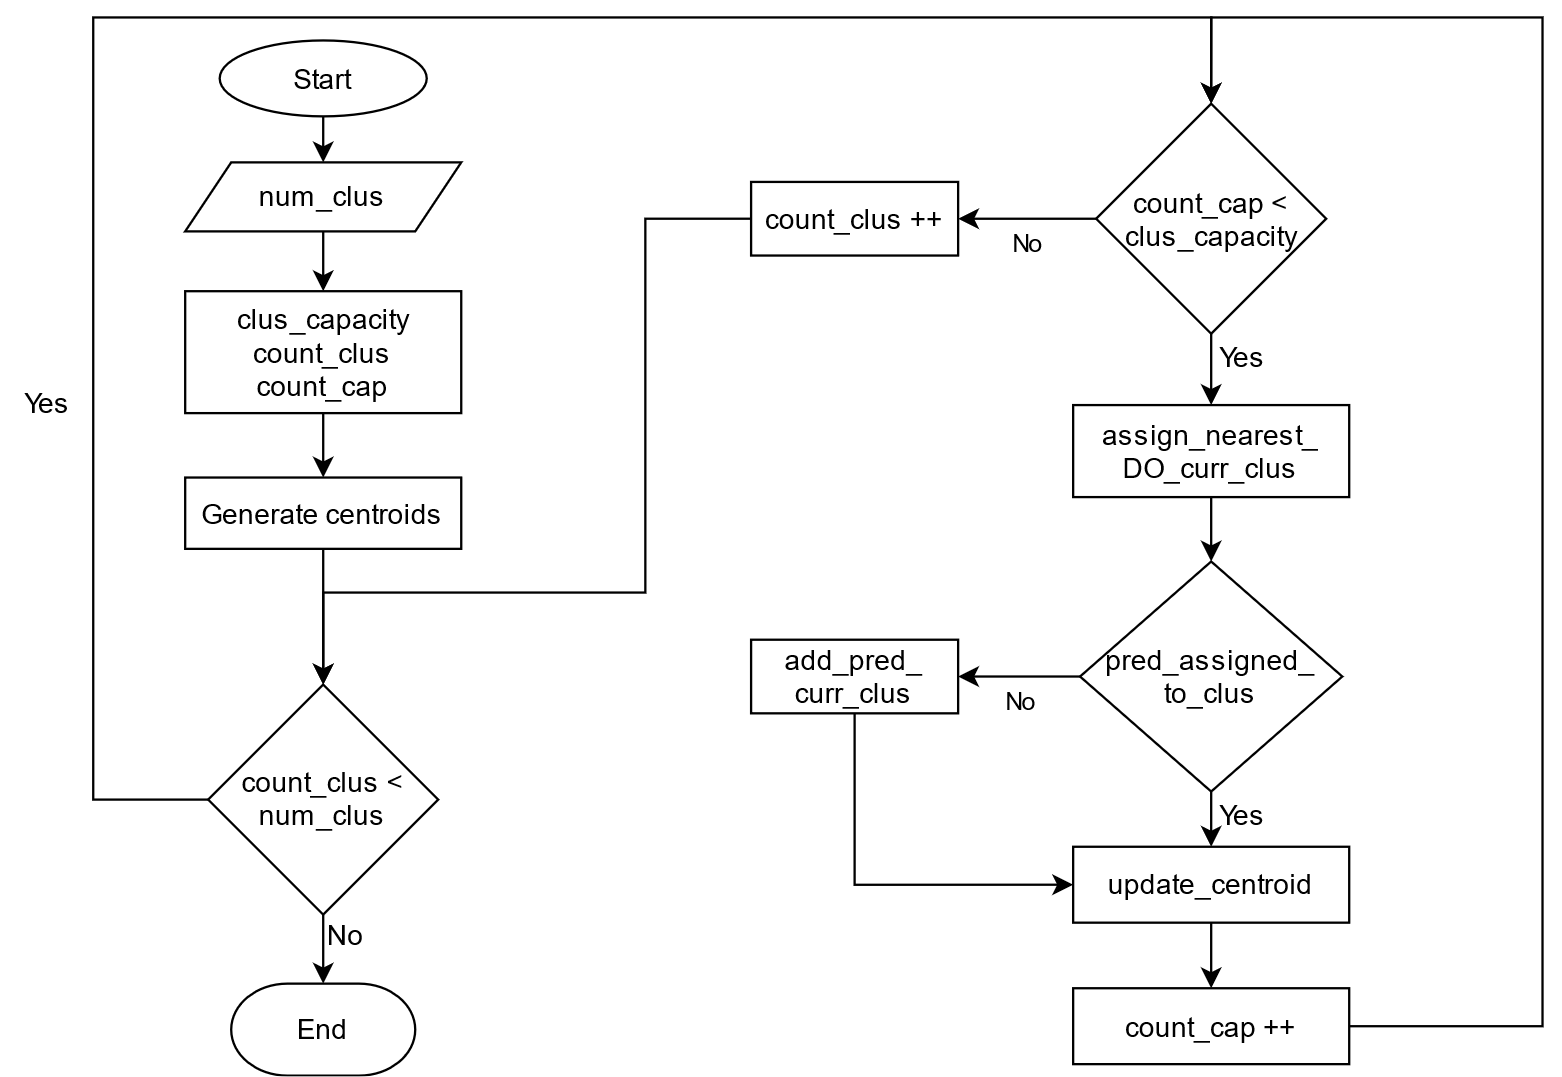
\includegraphics[width=\linewidth]{Flow_chart_9.png}
  \caption{Flowchart of the proposed Clustering Algorithm.}
  \label{fig1}
\end{figure}
\fi

%\newpage

\section{Results}
\label{sec:eval}
We use the benchmark instances presented in \cite{taillard1993benchmarks} as a dataset to work on. Many researchers have studied these instances and presented different approaches to solving them. We also developed different decomposition strategies to solve those. Therefore, it will be possible to measure the success/failure of our proposed model by comparing the results of the strategies developed in the past with those obtained from the proposed algorithm. There are 12 features, as we described in the previous section. In order to know which features have a significant effect on the results, we did some combinations of the features to perform the decomposition process clustering-based and then solved the problem using the Answer Set Programming model developed in \cite{el2020job} with a timeout of 10 minutes. We started with a simple combination that consists of $3$ features; \stfifo, \stmtwr, and \stest. At each step, we added another feature to get a new combination. The combinations of the selected features are listed as follows:
\begin{enumerate}
\fontsize{9pt}{10pt}
\item \textbf{F1} \textrightarrow \textit{\{ \stfifo, \stmtwr, \stest \}}
\item \textbf{F2} \textrightarrow \textit{\{ \stfifo, \stmtwr, \stest, RPT \}}
\item \textbf{F3} \textrightarrow \textit{\{ \stfifo, \stmtwr, \stest, EST \}} 
\item \textbf{F4} \textrightarrow \textit{\{ \stfifo, \stmtwr, \stest, ML \}} 
\item \textbf{F5} \textrightarrow \textit{\{ \stfifo, \stmtwr, \stest, RPT, EST \}}
\item \textbf{F6} \textrightarrow \textit{\{ \stfifo, \stmtwr, \stest, RPT, ML \}} 
\item \textbf{F7} \textrightarrow \textit{\{ \stfifo, \stmtwr, \stest, EST, ML \}} 
\item \textbf{F8} \textrightarrow \textit{\{ \stfifo, \stmtwr, \stest, \wtfifo, \wtmtwr, \wtest \}} 
\item \textbf{F9} \textrightarrow \textit{\{ \stfifo, \stmtwr, \stest, \wtfifo, \wtmtwr, \wtest, RPT \}} 
\item \textbf{F10} \textrightarrow \textit{\{ \stfifo, \stmtwr, \stest, \wtfifo, \wtmtwr, \wtest, EST \}} 
\item \textbf{F11} \textrightarrow \textit{\{ \stfifo, \stmtwr, \stest, \wtfifo, \wtmtwr, \wtest, ML \}}
\item \textbf{F12} \textrightarrow \textit{\{ \stfifo, \stmtwr, \stest, \wtfifo, \wtmtwr, \wtest, RPT, EST \}}
\item \textbf{F13} \textrightarrow \textit{\{ \stfifo, \stmtwr, \stest, \wtfifo, \wtmtwr, \wtest, RPT, ML \}}
\item \textbf{F14} \textrightarrow \textit{\{ \stfifo, \stmtwr, \stest, \wtfifo, \wtmtwr, \wtest, EST, ML \}}
\item \textbf{F15} \textrightarrow \textit{\{ \stfifo, \stmtwr, \stest, \wtfifo, \wtmtwr, \wtest, RPT, EST, ML \}}
\end{enumerate}
We neglected the rank of an operation and the time length of a job because they had negative impact results from the preliminary experiments. The following Table~\ref{tab4} shows the selected features, and the performance of each combination for solving benchmark instances of 50 jobs and 15 machines \cite{taillard1993benchmarks}. The following table shows the results of our experiments. The first column shows the approaches used for solving the problem in the literature in addition to the combinations of features we presented previously. The next columns represent the instances of our benchmark set except for the last column, which shows the average of each approach through the whole benchmark set. The first $4$ rows in the table show the values of each makespan obtained by heuristics; FIFO, MTWR, and (EST with a single and multi-shot). We can say that FIFO and MTWR provided the best results compared to the other two heuristics. However for the features combinations, the combinations (\textbf{F6}, \textbf{F8}, \textbf{F11}, \textbf{F12}and \textbf{F15}) provided good results according to the cost function in the most cases especially with combinations (\textbf{F6} and \textbf{F15}). It means that the most important features extracted from the problem itself and have a positive impact on the performance are \textit{Remaining Processing Time, Machine Load and Earliest Starting Time}. Also, The information obtained from the solutions of the other heuristics like (\textit{Starting Time} and \textit{Waiting Time}) led us to get better decomposition for the problem at hand. More specifically, combining \textit{Remaining Processing Time} with \textit{Machine Load} provides a good decomposition with/without \textit{Waiting Time} attributes obtained by the other heuristics. In a few instances, our proposed method did not outperform other heuristics, however, in the last column, the best average makespan of the other approaches was $3331$ by FIFO, and the average makespan of our feature selection algorithm was $3256$. We can conclude that the feature selection algorithm outperformed other heuristics in the literature. The following section illustrates the difference between our proposed algorithm and the methods implemented by other researchers.

\begin{table}
  \begin{center}
    \caption{The performance of selected features.}
    \label{tab4}

    \begin{tabular}{|l|l|l|l|l|l|l|l|l|l|l|l|} \hline
      & \multicolumn{11}{|c|}{\textbf{Instances}} \\ \cline{2-12}
      \textbf{Approach}   & TA51                           & TA52                           & TA53                           & TA54 & TA55                           & TA56                           & TA57                           & TA58 & TA59                           & TA60 & AVG  \\ \hline
      \textbf{FIFO}        & 3549                           & 3339                           & \textbf{3160}              & \textbf{3218} & 3291               & 3325                           & 3654                           & \textbf{3299} & \textbf{3344}                           & \textbf{3129} & \textbf{3331} \\
      \textbf{MTWR}        & \textbf{3364}           & \textbf{3304}              & 3168                           & 3494 & \textbf{3237}                           & \textbf{3287}               & \textbf{3633}              & 3591 & 3394                           & 3257 & 3373 \\
      \textbf{Single-shot} & 3632                           & 3615                           & 3481                           & 3462 & 3552                           & 3610                           & 3778                           & 3718 & 3613                           & 3550 & 3601 \\
      \textbf{EST}         & 3506                           & 3773                           & 3478                           & 3497 & 3482                           & 3605                           & 3753                           & 3731 & 3398                           & 3247 & 3547 \\ \hline
      \textbf{F1}          & 3506                           & 3277                           & 3382                           & 3414 & 3308                           & 3353                           & 3605                           & 3352 & 3453                           & 3483 & 3413 \\
      \textbf{F2}          & 3362                           & 3318                           & 3585                           & 3425 & 3441                           & 3380                           & 3573                           & 3412 & 3416                           & \textbf{3315} & 3423 \\
      \textbf{F3}          & 3324                           & 3330                           & 3347                           & 3425 & 3424                           & 3548                           & 3601                           & 3370 & 3301                           & 3617 & 3429 \\
      \textbf{F4}          & 3360                           & 3286                           & 3543                           & 3503 & 3319                           & 3270                           & 3583                           & 3509 & 3339                           & 3563 & 3428 \\
      \textbf{F5}          & 3346                           & 3243                           & 3517                           & 3397 & 3355                           & 3383                           & 3650                           & 3707 & 3508                           & 3591 & 3470 \\
      \textbf{F6}          & \textbf{3294} & 3275                           & 3250                           & 3265 & 3386                           & 3366                           & \textbf{3480} & \textbf{3324} & 3430                           & 3327 & \textbf{3340} \\
      \textbf{F7}          & 3328                           & 3226                           & 3338                           & 3353 & 3301                           & 3564                           & 3592                           & 3496 & 3352                           & 3399 & 3395 \\
      \textbf{F8}          & 3588                           & 3397                           & 3251                           & 3563 & 3498                           & \textbf{3229} & 3621                           & 3517 & 3258                           & 3374 & 3430 \\
      \textbf{F9}          & 3588                           & 3373                           & 3522                           & 3443 & 3385                           & 3306                           & 3543                           & 3716 & 3381                           & 3526 & 3475 \\
      \textbf{F10}         & 3568                           & 3533                           & 3373                           & 3386 & 3530                           & 3362                           & 3608                           & 3644 & 3402                           & 3637 & 3504 \\
      \textbf{F11}         & 3514                           & 3256                           & 3585                           & 3352 & 3365                           & 3344                           & 3670                           & 3611 & \textbf{3145} & 3425 & 3427 \\
      \textbf{F12}         & 3682                           & 3494                           & \textbf{3143} & 3270 & 3309                           & 3332                           & 3632                           & 3471 & 3250                           & 3676 & 3426 \\
      \textbf{F13}         & 3624                           & 3505                           & 3427                           & 3236 & 3370                           & 3338                           & 3749                           & 3437 & 3253                           & 3659 & 3460 \\
      \textbf{F14}         & 3554                           & 3373                           & 3524                           & \textbf{3232} & 3385                           & 3483                           & 3573                           & 3365 & 3284                           & 3767 & 3454 \\
      \textbf{F15}         & 3509                           & \textbf{3184} & 3380                           & 3289 & \textbf{3218} & 3389                           & \textbf{3480} & 3481 & 3290                           & 3569 & 3379 \\ \hline
      \textbf{Obtained} & 3294                           & 3184 & 3143                           & 3232 & 3218 & 3229                           & 3480 & 3324 & 3145                           & 3315 & \textbf{3256} \\
\hline
      \end{tabular}
  \end{center}
\end{table}



\section{Related Work}
\label{sec:literature}
In this section, we will review some of the most related works about data mining approaches employed to solve scheduling problems. Over the last decades, solving the scheduling problem has attracted the interest of many researchers, and a wide range of approaches has been developed for solving the scheduling problem. One of the approaches that have been widely used to solve the problem is data mining. The main idea of data mining is to explore the patterns from the obtained solutions by some heuristics and then develop some decision rules that approximate the order of the operations in each machine \cite{ismail2012production}. More precisely, it aims to get an order of the operations according to some characteristics.\\

Data mining methodologies are applied to explore the patterns in data generated by Genetic Algorithm (GA) \cite{koonce2000using}. This work aimed to generate rules to determine the priority for each job with weight. They solved the scheduling problem using GA to create some rules. Some characteristics (rank of operations, processing time, machine load, and remaining processing time) have been considered. In order to evaluate their heuristic, they tested the generated rules on some other instances that were randomly generated. The results showed that the generated rules were able to outperform the shortest processing time heuristic. One of the drawbacks is that the problem instances considered contain only 36 operations.\\

Other researchers also implemented GA to get some information of the solution but considered other features to generate decision rules \cite{harrath2002genetic}. They considered processing time, job length, remaining processing time, the rank of the operation, and machine load. To build a generic model for scheduling problems, they discretized the data by converting the quantitative data into qualitative. They sorted the operations share the same machine according to processing time. If two or more operations have the same processing time, they look at the time length of the job. If the job length is the same, sort them out based on the remaining processing time.\\

The work mentioned above had considered static JSP. However, dynamic JSP became one of the most crucial problems in real-life applications. New dispatching rules for JSP are presented using a data mining approach to obtain an efficient schedule in a dynamic Job-shop Scheduling environment \cite{shahzad2010discovering}. This study aimed to minimize makespan by creating new dispatching rules. Firstly, they solved the scheduling problems using Tabu Search and used the obtained solution as a training set to get a rule-set capable of approximating efficient solutions. They considered some other features like (Earliest possible Starting Time EST, the difference in remaining processing time for a job, and the difference in the processing time of two operations) to create a rule-set for dispatching the operations. The experiments showed that the results of mined rule-set are superior or comparable to the heuristics in the literature.\\

The variable neighborhood search (VNS) is combined with the k-means algorithm to address Dynamic JSP \cite{adibi2014clustering}. The proposed algorithm depends on extracting information from the problem's input data when an event like (machine breakdown or adding new job(s)) occurred. At any rescheduling point, cluster analysis is performed to replace jobs according to their distances. In other words, a job that belongs to a farther cluster has a greater probability to be selected in making a new adjacent than the other belonging to a closer cluster. The proposed method was compared to VNS and some common heuristics using a simulated job shop. the results indicated that the performance of the proposed model is better than the others, including some heuristics (FIFO, LIFO, and SPT).\\

Another study has presented a data mining approach to generate an initial population for population-based heuristics/metaheuristics to solve JSP \cite{nasiri2019data}. They extracted information from optimal or near-optimal solutions obtained by a heuristic procedure called "Assignment Procedure" to build decision rules to determine the priority of the operations. Once the rules are extracted, the initial solution is generated using these rules. To evaluate the performance of the proposed method, they performed a series of computational experiments on several test instances. The results showed that the proposed method with data mining generated initial population outperforms the methods with randomly generated initial population.\\

From the literature, we have found that most of the studies which used data mining techniques aimed to extract some features either from the problem instances or solutions obtained by some heuristics to build a decision-rules to order the operations assigned to a machine.\\


\section{Conclusions}
\label{sec:conclusions}
Data mining and machine learning is an area of interest in many manufacturing companies and other fields. In order to increase productivity and decrease the operation cost, there should be high-quality schedules to be used. This study focused on data mining and clustering approaches for solving the Job-shop Scheduling Problem. The first issue in this work is to explore the knowledge in good schedules and try to use this knowledge to get more efficient schedules. We extracted some features from the problem at hand and other features from schedules obtained by heuristics. The second issue is finding a powerful way to decompose the problem into windows where each cluster is a window and solve them sequentially. In order to split the problem, we proposed a constrained clustering algorithm considering the precedence constraints of the JSP. We tested our model on benchmark instances, and the results showed that the performance of the proposed model outperforms other heuristics FIFO, MTWR, and EST in the most cases; and some attributes like (\textit{Starting Time, Waiting Time, Remaining Processing Time, and Machine Load}) played an important role to split the operations in a good way. There are several ways to extend this study. Firstly, solve bigger instances and others in a real-life application in which more features could be extracted. Secondly, develop other clustering algorithms to split the problem more efficiently and get better results.

\bibliographystyle{splncs04}
\bibliography{references}


\end{document}
